\chapter{Introduction}

\section{Motivation}
Carbonaceous nanoparticles are widely encountered in nature and engineering. Every year, nearly 9.5 megatons of soot (black carbon) is emitted into the atmosphere from anthropogenic activities and natrual sources such as wildfires and volcanoes. The wide absorption range of soot reduces the albedo of snow-covered area and alters the radiative forcing balance in the atmosphere making soot the third strongest contributor to climate change after methane and carbon dioxide~\citep{myhre2014anthropogenic}. Also, exposure to combustion-generated soot could promote respiratory and cardiovascular disease ~\citep{world2013health}. So, strict regulations are targeting combustion engines to limit environmental and health risks from soot formation~\citep{integrated2019}. Accurate and affordable models are essential for the prediction of soot composition and morphology in combustion devices that helps reducing the emissions in engines. They can also provide better understanding of soot optical properties that are major indicator of soot environmental effects.

On the other hand, Carbon black (CB) with a similar synthesis process and structure to soot but higher elemental carbon to hydrogen ratios ($>$97\%)~\citep{watson2001carbon} is commercially produced and sold in large scales. In fact, CB is the largest industrially produced nanomaterial by value and volume (\~15 megatons per year with a value of \$17B) with applications as a reinforcing agent in rubber and tire industries~\citep{international2016carbon} and conductive additive in lithium-ion batteries~\citep{Palomares2010}. Carbon Black is primarily manufactured by the so-called furnace process where about 50\% of heavy fuel oil is partially combusted to convert the rest of it into CB~\citep{pratsinis2011history}. This process suffers from low mass yield and excessive emission, generating 4 tons of CO2 per each ton of product on average~\citep{bansal1993carbon}. Plasma reactor is an emerging alternative production method with distinct advantages over flame-based methods: They can achieve 100\% carbon yields with no direct emission of $\mathrm{CO_2}$ or other pollutants such, SOx or NOx~\citep{cho2004conversion}, and the energy required for pyrolysis is supplied by an electric arc that does not depend on the feedstock composition. Controlling CB properties such as its specific surface area (or primary particle diameter), hard agglomerate size (or gyration diameter of agglomerates with primary particles connected to each other by strong chemical bonds), and composition (or particle carbon to hydrogen ratio) is important make process economical and to achieve specific grades of CB for different target applications. However, this is a challenging task because of the complexity of CB formation and mass growth processes and its coupling with gas phase chemistry coupling with chemistry, dependence on local temperature and pressure. This requires accurate process design and optimization tools that provides insight into CB formation and evolution process, and inform manufacturer's decisions to adjust to produce CB with desired grades~\citep{park2005influence}.
 
The term \textit{"soot}" usually refers to unwanted particulate matter formed during combustion of any carbon-containing material from jet and diesel fuel to wood, heavy oil, and plastics with variable organic content and large H/C ratios~\citep{watson2001carbon}, but this research focuses on soot particles generated under controlled laboratory conditions from fuels with known compositions. The mature soot formed in methane and ethylene premixed flame can reach 95\% elemental C/H ratio~\cite{russo2015dehydrogenation}, which is close to CB composition. The comparison of the TEM images of industrially produced CB~\citep{singh2018nanostructure} with soot from diesel fuel~\citep{vander2007hrtem, lapuerta2017morphological} indicates similarity of their morphology and structure. Hereafter, soot is used to describe carbonaceous nanoparticels produced in flame/reactor during combustion/pyrolysis.

\begin{figure}[!htbp]
	\centering
	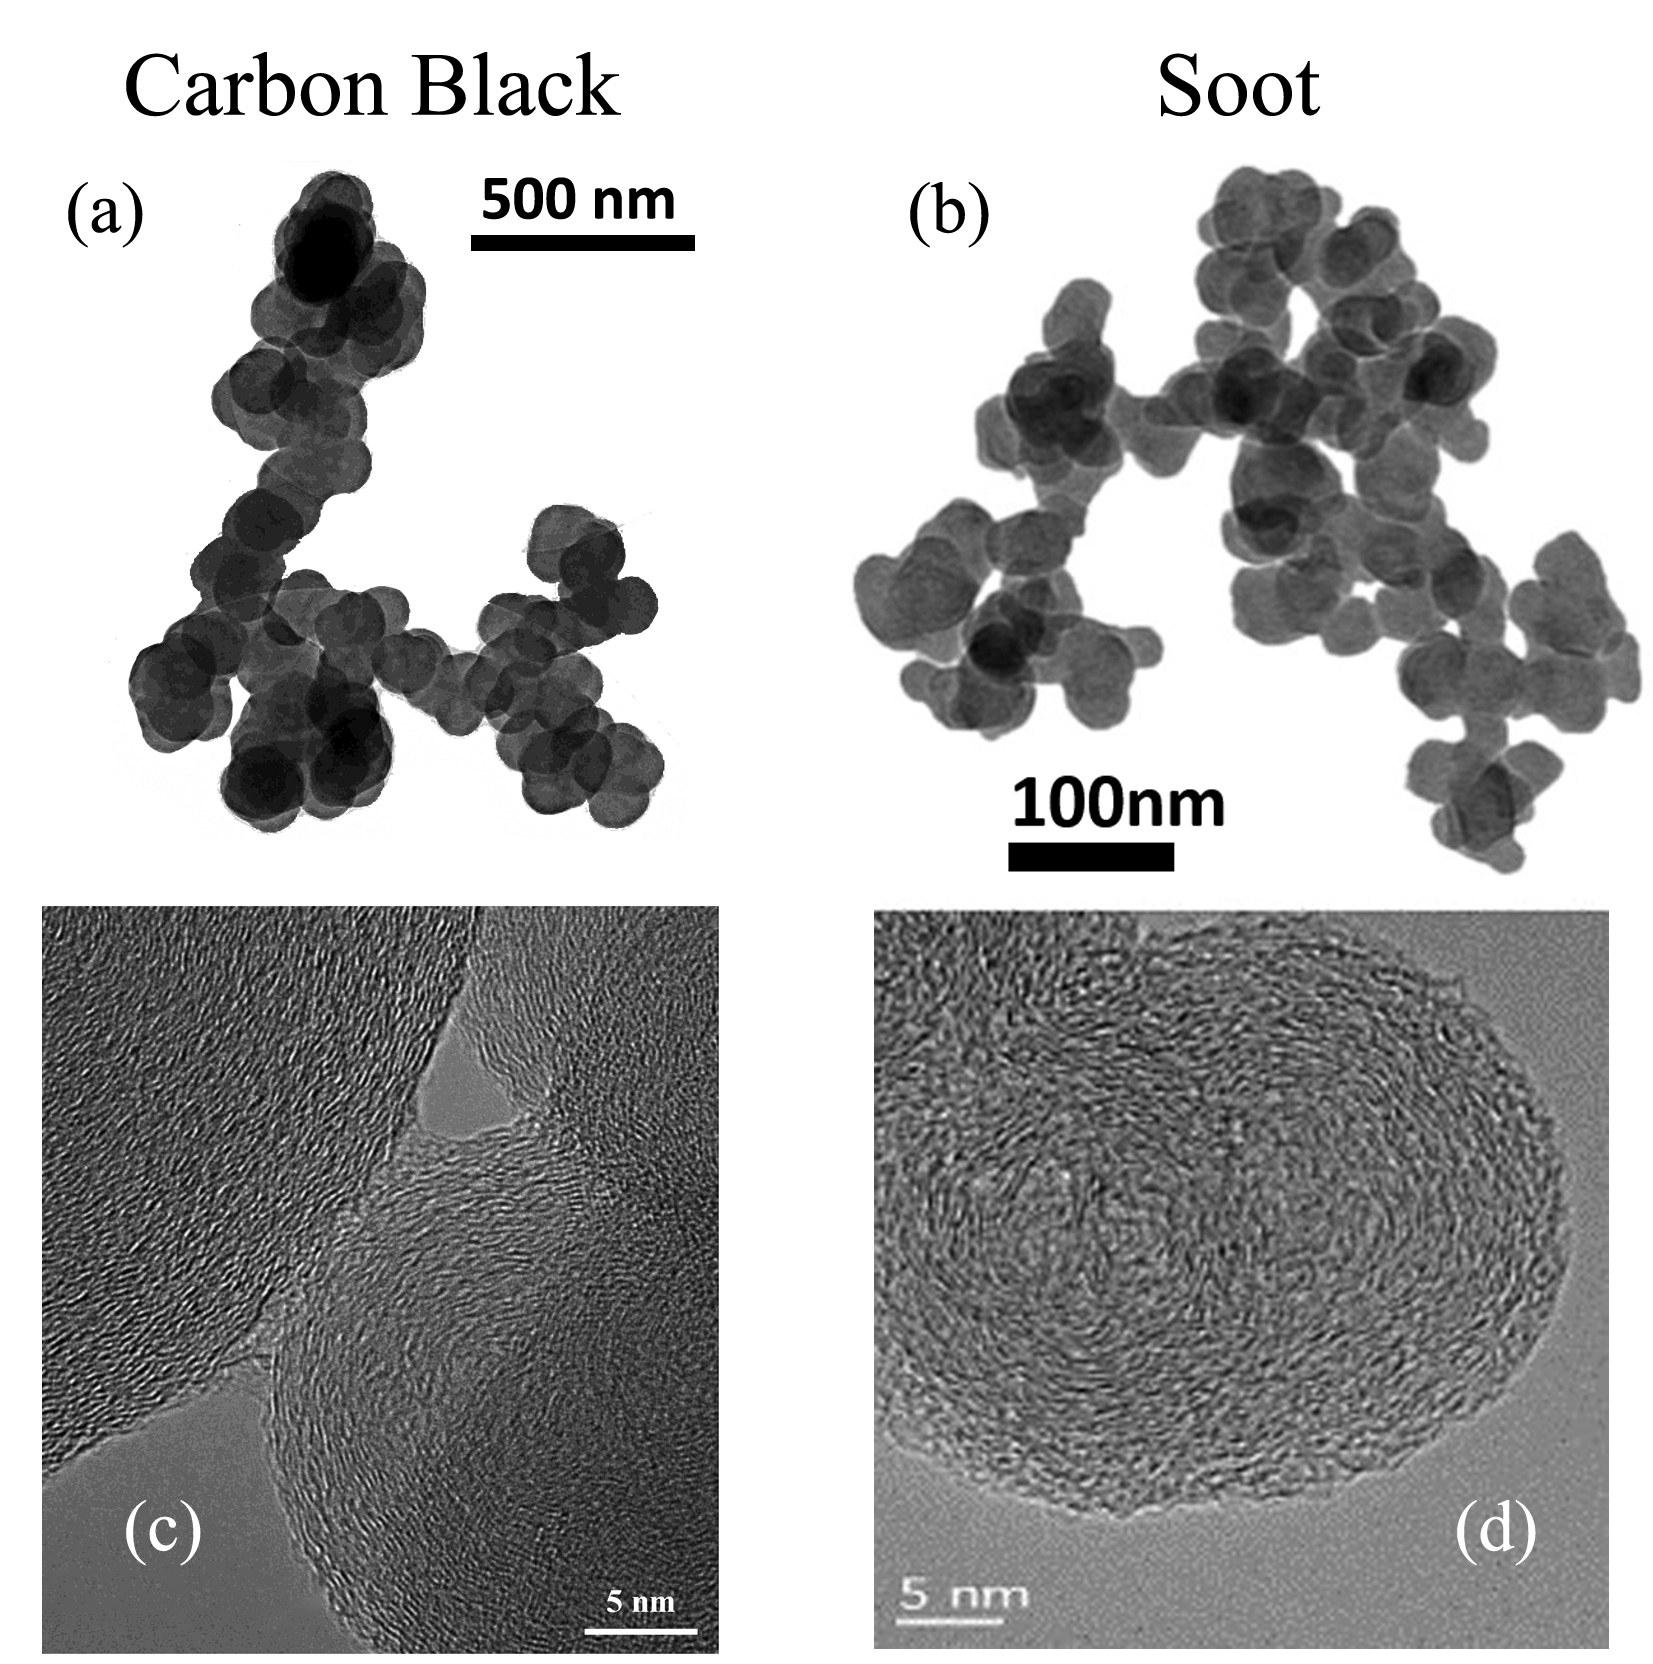
\includegraphics[height=60mm, ]{Figures/Introduction/soot_CB_HRTEM.jpg}
	\caption{The TEM images of Carbon black (a \& c)~\citep{singh2018nanostructure} and soot (b \& d)~\citep{vander2007hrtem, lapuerta2017morphological}}
	\label{fig:sootCBHRTEM} that shows soot and CB has similar morphology and structure
\end{figure} 


\section{Background}
\subsection{Soot inception and growth}
Soot formation is a complex process which involves gas chemistry, gas-to-solid transition, heterogeneous reactions on solid particles, and aerosol dynamics~\citep{d2009combustion}. It start form inception which refers to birth of the new soot particles known as incipient soot. The physics of soot inception is still elusive due to coupling with gas chemistry~\cite{Wang2011}, dependence on local temperature~\citep{gleason2018effect} and pressure~\cite{gleason2021pahs}. It has also been challenging to pinpoint the start of inception because of its short-time scales in the order $10^{-9}$ s~\citep{buesser2012design}, the lack of a decisive criterion to distinguish molecules from particles~\citep{d2009combustion}, and the overlap of inception with particle growth and agglomeration~\cite{martin2022soot}. Despite these limitations and challenges, our knowledge about soot formation has significantly increased thanks for advances in diagnostics methods and reaction mechanism development. 

There is compelling evidence that highlights the role of Polycyclic Aromatic Hydrocarbons (PAH) as the main soot precursors. They are thermodynamically stable enough to withstand dissociation at high flame temperatures~\citep{stein1985high} and observed in stacked layers in High Resolution Transmission Electron Microscope (HRTEM) images of soot primary particles~\citep{Oberlin1984}. But, the two important questions need to be answered: (1) which PAHs contribute most to the inception, and (2) what pathways best describe PAH to incipient soot transition. Purely chemical growth mechanisms are shown to underpredict inception rates and particle size~\citep{frenklach2002reaction}. The bimodality of particle size distribution in premixed flames~\citep{camacho2015mobility} suggests a mechanism second order with respect to the monomer~\citep{Wang2011}. To satisfy these requirements, a collision-based inception was proposed where irreversible polymerization form PAH clusters held together by Van der Wales forces. The theory postulates that PAH growth continues to reach a certain mass threshold that marks emergence of solid particles, but for practical purposes, a dimer is usually considered as incipient soot. 

In this model, hereafter referred to as \textbf{Irreversible Dimerization}, the collision of two PAH results are assumed to form a dimer that gain mass via two growth mechanisms: (i) hydrogen-abstraction-carbon-addition (HACA) that assumes soot surface to consist of hydrogenated sites with predefined density that can lose hydrogen and react with acetylene (ii) collision of PAH molecules/clusters with soot particles leading to adsorption. Irreversible Dimerization has been used to predict soot formation in burner-stabilized premixed~\citep{salenbauch2015modeling, desgroux2017comparative}, counterflow diffusion flames~\citep{wang2015soot, xu2021experimental}, coflow diffusion flames~\citep{kholghy2016core, veshkini2016understanding}. A collision efficiency factor ranging between $10^{-6}$ to 1 is also employed to adjust the inception flux and PAH adsorption rates to achieve desired soot mass and size distribution. PAHs of moderate sizes such as pyrene (4 rings) to coronene (7 rings) have been considered as the starting point of inception due to their thermodynamic instability that justifies the irreversibility at high temperatures~\citep{frenklach1991detailed}. However, the theoretical calculations~\citep{miller1985calculations} and experiments~\citep{sabbah2010exploring} indicated that pyrene dimerization is highly reversible in flame condition.

%While, this approach can describe inception in low to moderate temperature (<1000 K), and adjusts the inception flux , but it cannot explain how physically-bonded dimers withstand fragmentation at high flame temperatures (>1000 K).      The initial simple The initial PAH classic dimerization describes the inception by physical collision of PAH molecules that  

% 




